% ****** Start of file apssamp.tex ******
%
%   This file is part of the APS files in the REVTeX 4.2 distribution.
%   Version 4.2a of REVTeX, December 2014
%
%   Copyright (c) 2014 The American Physical Society.
%
%   See the REVTeX 4 README file for restrictions and more information.
%
% TeX'ing this file requires that you have AMS-LaTeX 2.0 installed
% as well as the rest of the prerequisites for REVTeX 4.2
%
% See the REVTeX 4 README file
% It also requires running BibTeX. The commands are as follows:
%
%  1)  latex apssamp.tex
%  2)  bibtex apssamp
%  3)  latex apssamp.tex
%  4)  latex apssamp.tex
%
\documentclass[%
 reprint,
%superscriptaddress,
%groupedaddress,
%unsortedaddress,
%runinaddress,
%frontmatterverbose, 
%preprint,
%preprintnumbers,
%nofootinbib,
%nobibnotes,
%bibnotes,
 amsmath,amssymb,
 aps,
%pra,
%prb,
%rmp,
%prstab,
%prstper,
%floatfix,
]{revtex4-2}

\usepackage{booktabs}
\usepackage{graphicx}% Include figure files
\usepackage{dcolumn}% Align table columns on decimal point
\usepackage{bm}% bold math
\usepackage{enumitem}
\usepackage[mathlines]{lineno}% Enable numbering of text and display math
%\linenumbers\relax % Commence numbering lines

%\usepackage[showframe,%Uncomment any one of the following lines to test 
%%scale=0.7, marginratio={1:1, 2:3}, ignoreall,% default settings
%%text={7in,10in},centering,
%%margin=1.5in,
%%total={6.5in,8.75in}, top=1.2in, left=0.9in, includefoot,
%%height=10in,a5paper,hmargin={3cm,0.8in},
%]{geometry}
\usepackage[english, spanish, mexico, es-noitemize]{babel}
\usepackage[pdfusetitle, colorlinks]{hyperref}
\hypersetup{
    colorlinks=true,    % Colores en lugar de cajas
    linkcolor=gray,
    citecolor=black, % Color de los enlaces internos
    filecolor=gray,  % Color de los enlaces a archivos
    urlcolor=gray       % Color de los enlaces externos
}
%\usepackage[shortlabels, inline]{enumitem}
\usepackage{array}
%\usepackage{titlesec}
%\usepackage[titles]{tocloft}
%\usepackage{xcolor, xpatch, calc}
%\usepackage{graphicx, booktabs}
%\usepackage{pgfplots}
%\usepackage[outline]{contour}
%\usepackage[hang, labelfont=bf, labelsep=period, margin=0.5in]{caption}
\usepackage{subcaption}
%\usepackage{csquotes}
\usepackage{lipsum}
%\usepackage{blindtext}
\usepackage{amsmath}
\usepackage{graphicx}
%\usepackage{svg}
%\usepackage{booktabs}
%\usepackage{enumitem}
\usepackage{float}
\usepackage{listings}
\usepackage{xcolor}
\usepackage{listings}
\lstset{
  language=Python,
  basicstyle=\ttfamily\small,
  commentstyle=\itshape\color{gray},
  keywordstyle=\bfseries\color{blue},
  numbers=left,
  numberstyle=\tiny\color{gray},
  stepnumber=1,
  numbersep=5pt,
  backgroundcolor=\color{white},
  frame=single,
  breaklines=true,
  breakatwhitespace=false,
  captionpos=b,
  tabsize=2,
  showspaces=false,
  showstringspaces=false
}

\usepackage{appendix}


\begin{document}

\preprint{APS/123-QED}

\title{Proyecto Intermedio}% Force line breaks with \\

 
\author{M. Gallego}
\email{mibarriosg@unal.edu.co}
\author{J. Segura}
\email{jusegurag@unal.edu.co}
\author{A. Silva}
\email{ansilvav@unal.edu.co}
\affiliation{Introducción a la Computación Científica y de Alto Rendimiento [2015174]\\Universidad Nacional de Colombia\\ Departamento de Física - Bogotá D.C}%
\date{\today}% It is always \today, today,
             %  but any date may be explicitly specified
\begin{abstract}
\begin{description}
\item[Resumen] En este trabajo se 


\end{description}
\begin{description}
\item[Palabras clave] Percolación.

\end{description}
\end{abstract}

\maketitle

\section{Introducción}

El fenómeno de percolación es un modelo fundamental en física estadística y teoría de redes, con aplicaciones que abarcan desde la propagación de incendios forestales y epidemias hasta la conductividad de materiales porosos. En su forma más simple, el modelo de percolación representa un sistema en el cual cada sitio (o enlace) de una red es ocupado con cierta probabilidad $p$, y se estudia la formación de caminos conectados a través del sistema.

En este trabajo se considera el modelo de percolación por sitio en una malla bidimensional cuadrada de tamaño $L \times L$, donde cada celda se ocupa de forma independiente con probabilidad $p$. Dos celdas ocupadas se consideran conectadas si son vecinas en la dirección de von Neumann (norte, sur, este u oeste). A partir de estas conexiones se forman clusters o componentes conexas de celdas ocupadas.

Un aspecto central del modelo es la transición de fase que ocurre en el límite termodinámico ($L \to \infty$): existe un valor crítico de $p$, denotado $p_c$, por debajo del cual la probabilidad de que exista un cluster que atraviese el sistema es prácticamente nula, y por encima del cual la percolación ocurre casi con certeza. En este proyecto, se estudian tres aspectos fundamentales del comportamiento del sistema en función de $p$ y del tamaño $L$:

\begin{enumerate}
    \item La probabilidad de percolación, es decir la fracción de configuraciones en las que existe un cluster que conecta lados opuestos de la malla, ya sea en dirección vertical (de arriba a abajo) o horizontal (de izquierda a derecha).
    \item El tamaño promedio del cluster más grande para en función de la probabilidad $p$ para cada $L$.
    \item El efecto que tiene el nivel de optimización del compilador \texttt{-O} en el tiempo de computo en función del tamaño del sistema $L$.
\end{enumerate}

Dado el carácter probabilístico del modelo, las simulaciones se repiten ?? para cada valor de $p$, de $L$, y \texttt{-O} con el fin de obtener estimaciones precisas de las cantidades de interés. A partir de estas repeticiones se calculan promedios y desviaciones estándar, lo que permite evaluar la estabilidad y confiabilidad de los resultados.

Desde el punto de vista computacional, el código fue implementado en C++ siguiendo una estructura modular. Se utilizó un Makefile para automatizar tanto la ejecución del programa como el proceso de análisis del desempeño. Este análisis incluyó tareas como depuración, pruebas unitarias, medición de cobertura de código y perfilamiento, mediante \textit{targets} específicos, los cuales se describen en detalle en la sección de metodología.

\section{Metodología}

\subsection{Código base}

El programa se estructuró de manera modular en tres archivos principales:

\begin{itemize}
    \item \texttt{functions.h}: contiene las declaraciones de funciones y las inclusiones de librerías necesarias para el resto del programa.
    
    \item \texttt{functions.cpp}: implementa las funciones que permiten analizar la malla, entre ellas las funciones principales \texttt{hay\_cluster\_percolante()} y \texttt{dfs()}, encargadas de identificar y etiquetar los clústeres, así como de detectar si alguno de ellos es percolante. Estas funciones se describen con mayor detalle más adelante.
    
    \item \texttt{main.cpp}: actúa como punto de entrada del programa. Recibe por línea de comandos los parámetros \texttt{L} (dimensión de la malla), \texttt{p} (probabilidad de ocupación) y \texttt{seed} (semilla aleatoria). Con estos valores, genera una malla binaria aleatoria de tamaño representada en un vector unidimensional de tipo \texttt{bool} y longitud \texttt{LxL}. También inicializa un vector \texttt{etiquetas} con ceros, del mismo tamaño, para registrar la pertenencia de cada sitio a un clúster, una variable \texttt{tamano\_max} y un vector \texttt{percolantes} vacío que almacenará las etiquetas de los clústeres que percolan tras el llamado a la función \texttt{hay\_cluster\_percolante()}. Durante todo este proceso mide el tiempo de ejecución (tanto \textit{CPU time} como \textit{wall time}) e imprime finalmente por consola si hay percolación, el tamaño del clúster percolante más grande y los tiempos registrados.
    
\end{itemize}

Ahora, procedemos a explicar la lógica de las dos funciones principales en las que recae el programa:

La función \texttt{hay\_cluster\_percolante()} recibe como argumento el vector de la \texttt{malla}, el tamaño \texttt{L}, la variable \texttt{tamano\_max}, el vector \texttt{etiquetas} y el vector \texttt{percolantes}. Esta recorre los sitios ocupados de la primera fila y la primera columna de la malla de tamaño \texttt{LxL}. Si alguno de estos sitios aún no ha sido etiquetado (es decir, si su valor en el vector \texttt{etiquetas} es cero), se lanza una búsqueda en profundidad llamando a la función \texttt{dfs()}.

La función \texttt{dfs()} toma como entrada la posición inicial del sitio (\texttt{id}), el tamaño de la malla (\texttt{L}), una etiqueta entera única (\texttt{etiqueta}) para identificar el clúster actual, el vector binario de la malla (\texttt{malla}), un vector de etiquetas para marcar los sitios ya visitados (\texttt{etiquetas}), y cuatro referencias booleanas (\texttt{toca\_arriba}, \texttt{toca\_abajo}, \texttt{toca\_izquierda}, \texttt{toca\_derecha}) que se actualizan si el clúster llega a los bordes respectivos. La función \texttt{dfs()} explora todos los sitios conectados al sitio inicial (\texttt{id}) que están ocupados y aún no etiquetados, asignándoles la etiqueta correspondiente y devolviendo el tamaño total del clúster encontrado. 

De vuelta en \texttt{hay\_cluster\_percolante()}, si el clúster encontrado cumple la condición de tocar simultáneamente los bordes superior e inferior (\texttt{toca\_arriba \&\& toca\_abajo}) o izquierdo y derecho (\texttt{toca\_izquierda \&\& toca\_derecha}), se considera un clúster percolante. En tal caso, se actualiza la variable \texttt{tamano\_max} si el nuevo clúster es mayor a los previos, y se agrega su etiqueta al vector \texttt{percolantes}.

Opcionalmente, \texttt{main.cpp} puede llamar a la función \texttt{imprimir\_clusters()}, que exporta la malla etiquetada a un archivo \texttt{.txt}. En este archivo, los sitios no ocupados se marcan con \texttt{0}, los ocupados que no forman parte de clústeres percolantes con \texttt{1}, y los clústeres percolantes con etiquetas enteras crecientes a partir de \texttt{2}. Esta salida se utiliza para visualizar gráficamente los clústeres percolantes como se muestra en la Figura \ref{fig:cluster}.

Con esta estructura base del código, se procedió a realizar simulaciones sistemáticas. Para cada combinación de los parámetros \( L \), \( p \) y nivel de optimización, el programa se ejecutó 10 veces utilizando diferentes semillas aleatorias. Se consideraron cinco tamaños de malla: \( L = 32, 64, 128, 256, 512 \); treinta valores de \( p \) distribuidos entre 0 y 1, con mayor densidad (10 valores) en la región crítica entre 0.55 y 0.65; y cinco niveles de optimización del compilador: \texttt{-O0}, \texttt{-O1}, \texttt{-O2}, \texttt{-O3} y \texttt{-Ofast}.

\subsection{Automatización con Makefile}

Para automatizar las distintas tareas del proyecto, se implementó un archivo \texttt{Makefile} con múltiples \textit{targets}, cada uno diseñado para realizar una tarea específica relacionada con la compilación, ejecución, análisis y validación del código. A continuación se describe la funcionalidad de cada uno de estos comandos y su uso desde la línea de comandos:

\begin{itemize}
    \item \texttt{make analisis}: compila y ejecuta el código para todas las combinaciones de \( L \), \( p \) y niveles de optimización especificadas anteriormente, utilizando 50 semillas distintas. Los datos generados se procesan mediante un script en Python, que produce las gráficas en formato PDF presentadas en la sección de resultados.

    \item \texttt{make simul L=\dots\ p=\dots\ seed=\dots}: compila y ejecuta una simulación individual con los valores de \( L \), \( p \) y semilla aleatoria especificados. Posteriormente, genera una visualización del clúster percolante.
    
    \item \texttt{make test}: ejecuta pruebas unitarias utilizando la librería Catch2 sobre cuatro casos base: una malla completamente vacía (\( p = 0 \)), una malla completamente ocupada (\( p = 1 \)), una malla con una línea horizontal de unos (para verificar percolación horizontal) y una con una línea vertical (para verificar percolación vertical). Estas pruebas comprueban la detección correcta de clústeres percolantes y el cálculo de sus tamaños.
    
    \item \texttt{make debug}: compila el programa con banderas de depuración y lo ejecuta bajo GDB para facilitar el análisis detallado de errores.
    
    \item \texttt{make valgrind}: compila el programa con banderas de depuración y ejecuta Valgrind para detectar pérdidas de memoria o accesos inválidos en un caso de prueba.
    
    \item \texttt{make profile}: genera un informe de \textit{flat profiling} usando la herramienta \texttt{perf}, tanto para la versión optimizada como para una versión previa no optimizada del código, para el caso de probabilidad crítica (\( L = 128 \), \( p = 0.59271 \), \texttt{seed} = 10). Esta comparación se analiza en detalle en la sección de dificultades y optimizaciones.
    
    \item \texttt{make coverage}: ejecuta los casos de prueba y genera un reporte en formato HTML que muestra la cobertura del código utilizando \texttt{gcovr}.
    
    \item \texttt{make clean}: elimina archivos binarios, intermedios y temporales, incluyendo ejecutables, archivos \texttt{.gcda}, \texttt{.gcno}, \texttt{.txt}, \texttt{.pdf} y carpetas como \texttt{resultados} o \texttt{coverage}.

    \item \texttt{make report}: crea este informe a partir de un archivo latex y las figuras en fomato PDF en el repositorio.
    
\end{itemize}


\section{Resultados}

\subsection{Probabilidad de percolación}

\begin{figure}[H]
    \centering
    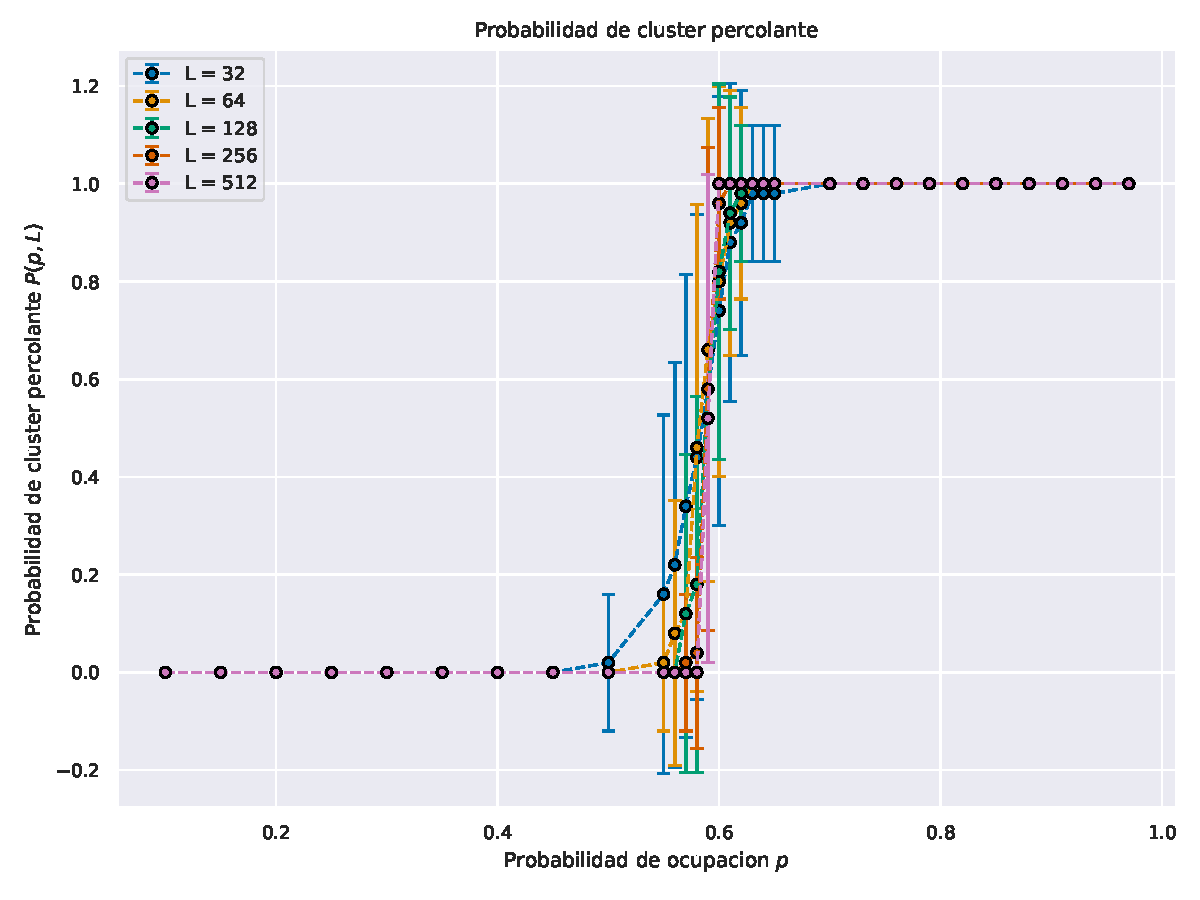
\includegraphics[width=1\linewidth]{ProbabilidadCluster.pdf}
    \caption{Caption}
    \label{fig:enter-label}
\end{figure}

\subsection{Tamaño promedio del cluster más grande}

\begin{figure}[H]
    \centering
    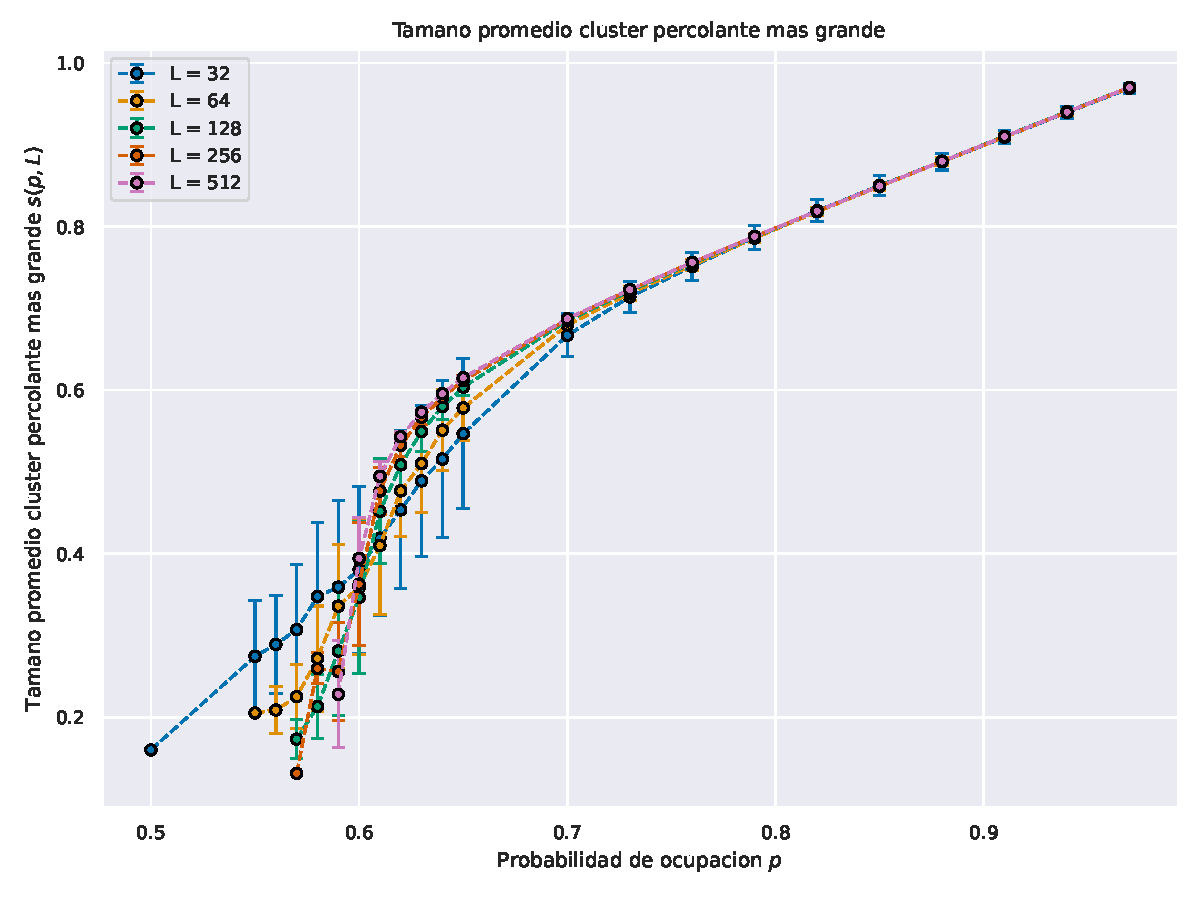
\includegraphics[width=1\linewidth]{TamanoCluster.pdf}
    \caption{Caption}
    \label{fig:enter-label}
\end{figure}

\subsection{Tiempo de computo para cada optimización}

\begin{figure}[H]
    \centering
    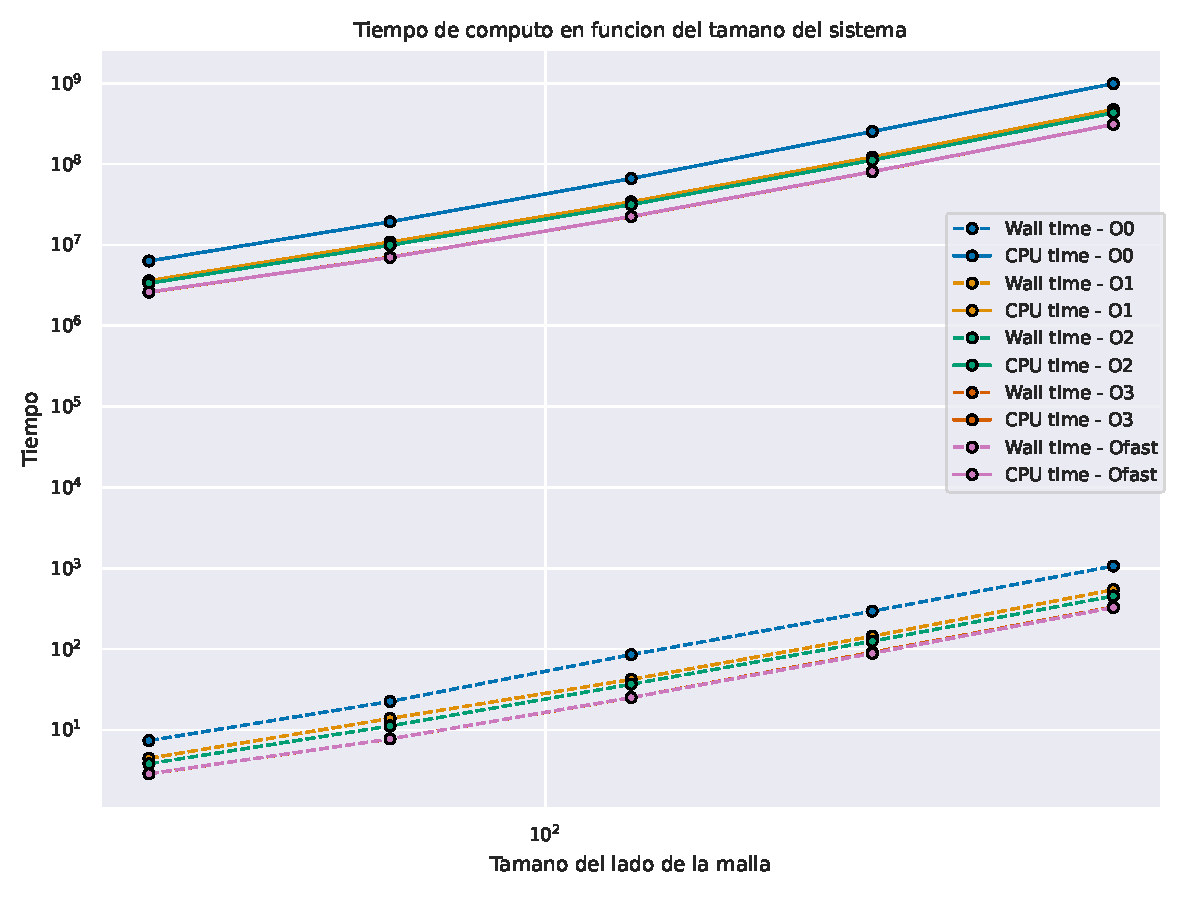
\includegraphics[width=1\linewidth]{Tiempos.pdf}
    \caption{Caption}
    \label{fig:enter-label}
\end{figure}

\subsection{Dificultades y optimizaciones}

Una de las principales dificultades encontradas durante el desarrollo del proyecto fue la implementación inicial de la función \texttt{dfs()}, la cual realizaba llamadas recursivas para explorar los vecinos de un sitio ocupado. Esta aproximación recursiva generaba un desbordamiento de pila (\textit{stack overflow}) en mallas grandes, como aquellas con \( L = 512 \), impidiendo que se completara la detección de clústeres percolantes y el cálculo de su tamaño.

La solución consistió en reemplazar la recursividad por una implementación iterativa utilizando un objeto \texttt{stack} de la biblioteca estándar \texttt{<stack>}. Esta estructura permitió gestionar explícitamente el recorrido por vecinos: se elimina el sitio actual de la pila y se agregan únicamente los vecinos ocupados y no etiquetados. Cuando la pila se vacía, se retorna el tamaño del clúster. Esta versión iterativa evita el desbordamiento y mejora el control del flujo de ejecución. La lógica completa está documentada mediante comentarios en \texttt{functions.cpp}.

Una vez resuelto este problema, se identificó una segunda optimización importante. La versión original de \texttt{hay\_cluster\_percolante()} evaluaba la conectividad para toda la malla (\( L \times L \)), lo cual era innecesariamente costoso para el objetivo de detectar si existe al menos un clúster percolante. Se observó que basta con explorar únicamente los sitios ocupados en la primera fila y la primera columna, ya que cualquier clúster percolante debe estar conectado a uno de estos bordes. Esta optimización redujo significativamente el tiempo de ejecución.

La mejora lograda puede observarse en los reportes de \textit{profiling} obtenidos con \texttt{perf} mostrados en la Figura \ref{fig:perf}, comparando dos versiones del código: una optimizada que solo recorre la primera fila y columna (\texttt{functions.cpp}), y otra sin optimización que recorre toda la malla (\texttt{functions\_viejo.cpp}). El caso analizado corresponde a los parámetros \( L = 128 \), \( p = 0.59271 \) y \texttt{seed} = 10.


\section{Conclusiones}

\bibliography{report}

\end{document}
%
% ****** End of file apssamp.tex ******